%###########################################################################
%
%   Anhang
%
%###########################################################################
\begin{appendix}
\ifthenelse{\equal{\Sprache}{0}}
{\chapter*{Anhang}\label{sec:Anhang}
	\setcounter{chapter}{1}
	\addcontentsline{toc}{chapter}{Anhang}
}{}
\ifthenelse{\equal{\Sprache}{1}}
{\chapter*{Appendix}\label{sec:appendix}
	\setcounter{chapter}{1}
	\addcontentsline{toc}{chapter}{Appendix}
}{}


%###########################################################################
%   Anhang A
%###########################################################################
\ifthenelse{\equal{\Sprache}{0}}
{\section{Inhalt Archiv}\label{sec:AnhangArchiv}
	\markboth{Anhang}{Anhang}
	%
	%
	Im Archiv ist ein Verzeichnis
\RemoveSpaces{
	\ifthenelse{\equal{\MScBSc}{0}}
	{\textbf{BSC$\_$\NummerDerArbeit$\_$\NachnameDesStudenten/}}{}
	\ifthenelse{\equal{\MScBSc}{1}}
	{\textbf{PRO$\_$\NummerDerArbeit$\_$\NachnameDesStudenten/}}{}
	\ifthenelse{\equal{\MScBSc}{2}}
	{\textbf{MSC$\_$\NummerDerArbeit$\_$\NachnameDesStudenten/}}{}
} abgelegt.
Dieses enthält in der obersten Dateistruktur die Einträge
	\begin{itemize}
	\item \ifthenelse{\equal{\MScBSc}{0}}
		{\textbf{BSC$\_$\NummerDerArbeit$\_$\NachnameDesStudenten.pdf}:}{}
		\ifthenelse{\equal{\MScBSc}{1}}
		{\textbf{PRO$\_$\NummerDerArbeit$\_$\NachnameDesStudenten.pdf}:}{}
		\ifthenelse{\equal{\MScBSc}{2}}
		{\textbf{MSC$\_$\NummerDerArbeit$\_$\NachnameDesStudenten.pdf}:}{}
		das pdf-File zur Arbeit
\RemoveSpaces{
		\ifthenelse{\equal{\MScBSc}{0}}
		{BSC-\NummerDerArbeit.}{}
		\ifthenelse{\equal{\MScBSc}{1}}
		{PRO-\NummerDerArbeit.}{}
		\ifthenelse{\equal{\MScBSc}{2}}
		{MSC-\NummerDerArbeit.}{}
}
		%
		\item \textbf{Daten/}: ein Verzeichnis mit den für diese Arbeit
		relevanten Daten, Hilfsprogrammen, Skripts und Simulationsumgebungen.
		\item \textbf{Latex/}: ein Verzeichnis mit den *.tex-Dateien des in
		Latex verfassten Berichts zur Arbeit
\RemoveSpaces{
		\ifthenelse{\equal{\MScBSc}{0}}
		{BSC-\NummerDerArbeit}{}
		\ifthenelse{\equal{\MScBSc}{1}}
		{PRO-\NummerDerArbeit}{}
		\ifthenelse{\equal{\MScBSc}{2}}
		{MSC-\NummerDerArbeit}{}
}
		sowie alle dazugehörigen Grafiken (falls vorhanden auch als *.svg Dateien).
		%
		\item \textbf{Vortrag/}: ein Verzeichnis mit den für den Vortrag relevanten Daten wie die Präsentation, Bilder und Videos.
		%
	\end{itemize}
}{}
\ifthenelse{\equal{\Sprache}{1}}
{\section{Contents Archive}\label{apx:archive}
	\markboth{Appendix}{Appendix}
	%
	%
	There is a folder
\RemoveSpaces{
	\ifthenelse{\equal{\MScBSc}{0}}
	{\textbf{BSC$\_$\NummerDerArbeit$\_$\NachnameDesStudenten/}}{}
	\ifthenelse{\equal{\MScBSc}{1}}
	{\textbf{PRO$\_$\NummerDerArbeit$\_$\NachnameDesStudenten/}}{}
	\ifthenelse{\equal{\MScBSc}{2}}
	{\textbf{MSC$\_$\NummerDerArbeit$\_$\NachnameDesStudenten/}}{}} in the archive. The main folder contains the entries
	\begin{itemize}
		\item \ifthenelse{\equal{\MScBSc}{0}}
		{\textbf{BSC$\_$\NummerDerArbeit$\_$\NachnameDesStudenten.pdf}:}{}
		\ifthenelse{\equal{\MScBSc}{1}}
		{\textbf{PRO$\_$\NummerDerArbeit$\_$\NachnameDesStudenten.pdf}:}{}
		\ifthenelse{\equal{\MScBSc}{2}}
		{\textbf{MSC$\_$\NummerDerArbeit$\_$\NachnameDesStudenten.pdf}:}{}
		the pdf-file of the thesis
\RemoveSpaces{
		\ifthenelse{\equal{\MScBSc}{0}}
		{BSC-\NummerDerArbeit.}{}
		\ifthenelse{\equal{\MScBSc}{1}}
		{PRO-\NummerDerArbeit.}{}
		\ifthenelse{\equal{\MScBSc}{2}}
		{MSC-\NummerDerArbeit.}{}}
		%
		\item \textbf{Data/}: a folder with all the relevant data, programs, scripts and simulation environments.
		\item \textbf{Latex/}: a folder with the *.tex documents of the thesis
\RemoveSpaces{
		\ifthenelse{\equal{\MScBSc}{0}}
		{BSC-\NummerDerArbeit}{}
		\ifthenelse{\equal{\MScBSc}{1}}
		{PRO-\NummerDerArbeit}{}
		\ifthenelse{\equal{\MScBSc}{2}}
		{MSC-\NummerDerArbeit}{}}
		written in Latex and all figures (also in *.svg data format if available).
		%
		\item \textbf{Presentation/}: a folder with the relevant data for the presentation including the presentation itself, figures and videos.
		%
	\end{itemize}
}{}

\clearpage
\section{Performance of MLRA and MLMPC in the Fully Observed Domain}\label{apx:fo-comparison}

The figures below illustrate the performance of \ac{mlra} and \ac{mlmpc} for
the fully observed version of the \ac{pomdp} formalized in
\cref{sec:lp-pomdp-formalization}. Notice that, \ac{mlmpc} is an optimal policy
for the fully observable motion planning problem. Thus, it achieves a $100\%$
success rate (\cf \cref{fig:lp_outcome_fo}) and the highest possible return
(\cf \cref{fig:lp_eval_undiscounted_fo,fig:lp_eval_infdiscounted_fo}).

\begin{figure}[htpb]
  \centering
  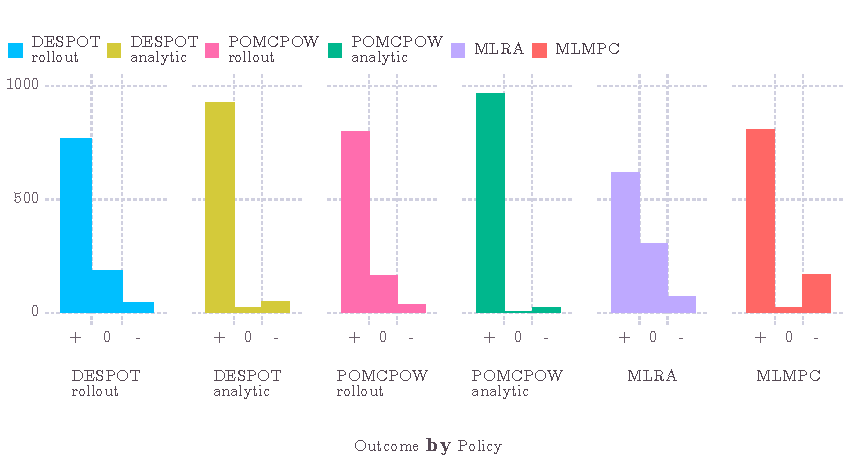
\includegraphics[scale=1.0]{roomba_plots/fully_observed/lp_outcome_eval_plot.pdf}
\caption{Histogram of outcome frequencies grouped by policy evaluated on the
         fully observed problem. Outcome classes: \emph{success (+)}, the robot
         reached the exit; \emph{failed to exit (0)}, the agent did not make it to the
         exit within the simulation horizon; and \emph{failure (-)}, the robot fell
         down the stairs.}
	\label{fig:lp_outcome_fo}
\end{figure}

\begin{figure}[htpb]
  \centering
  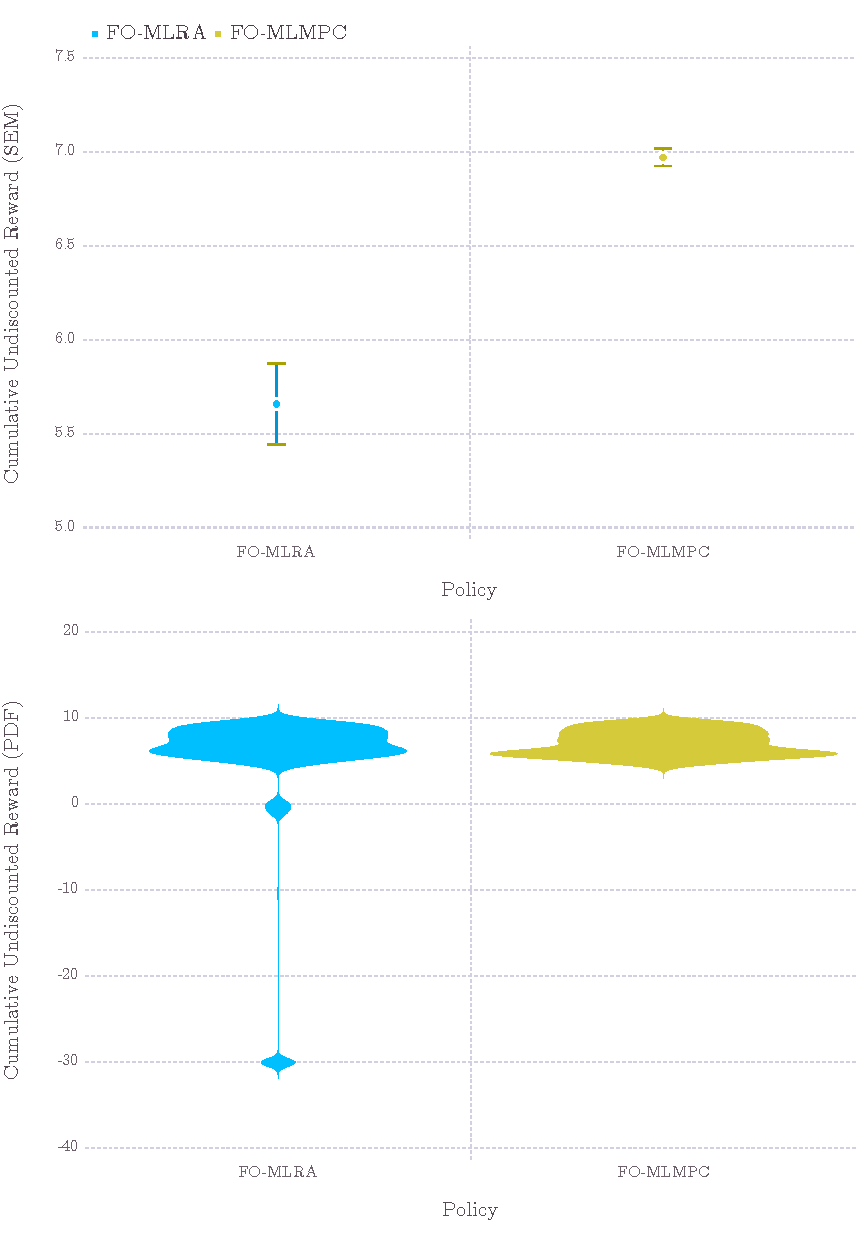
\includegraphics[scale=1]{roomba_plots/fully_observed/lp_value_eval_plot-undiscounted_reward.pdf}
  \caption{Statistics of the cumulative \emph{undiscounted} reward for each
           policy evaluated on the fully observed problem. Top: Mean and \acf{sem}.
           Bottom: Approximation of the \acf{pdf}.}
  \label{fig:lp_eval_undiscounted_fo}
\end{figure}

\begin{figure}[htpb]
  \centering
  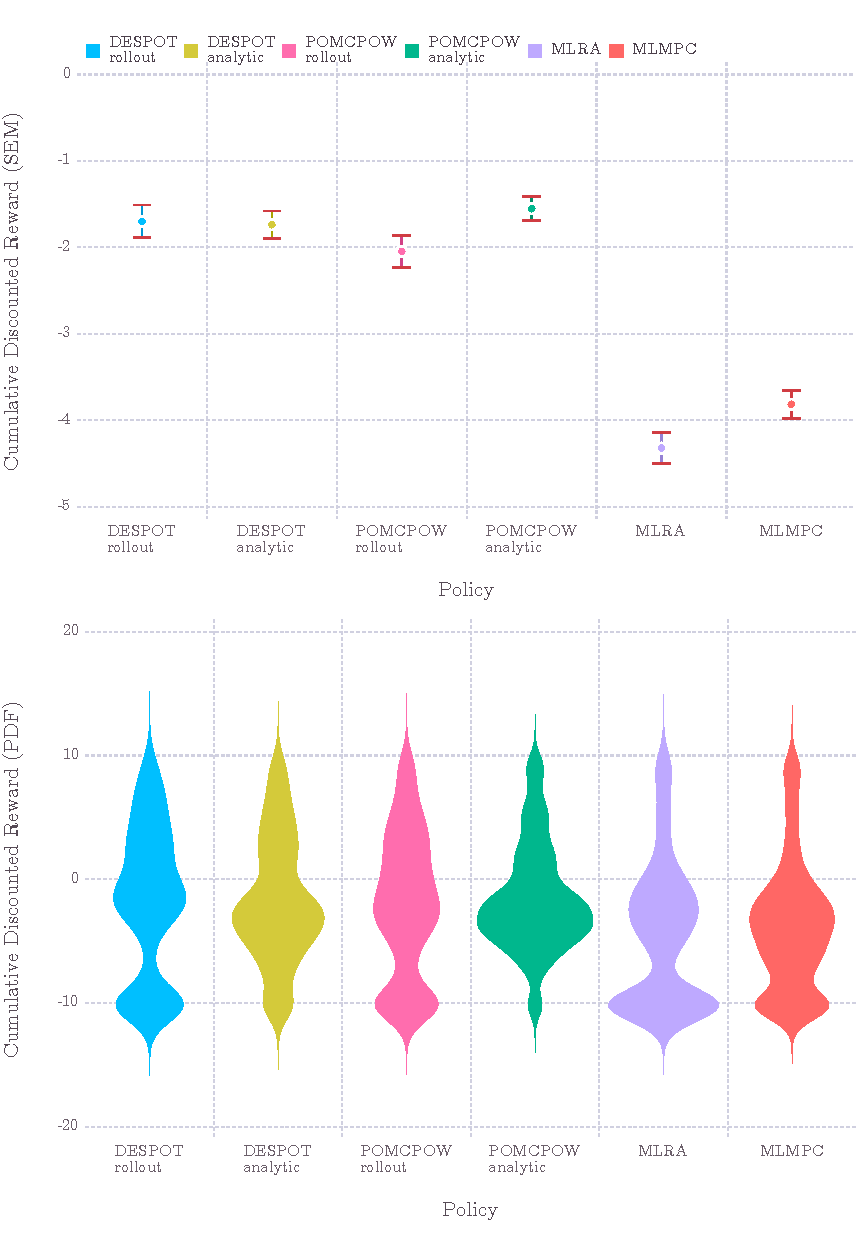
\includegraphics[scale=1]{roomba_plots/fully_observed/lp_value_eval_plot-inf_discounted_reward.pdf}
  \caption{Statistics of the cumulative \emph{discounted} reward for each
           policy evaluated on the fully observed problem. Top: Mean and \acf{sem}.
           Bottom: Approximation of the \acf{pdf}.}
  \label{fig:lp_eval_infdiscounted_fo}
\end{figure}

\clearpage

\section{Example Trajectories for \cref{chap:localization-and-planning}}\label{apx:lp-example-trajectories}

\Crefrange{fig:pomcpow-analytic-infogather}{fig:mlmpc-oscillating} show example
trajectories visualizing the qualitative difference between active and passive
information gathering. In this example, active information gathering allows
\ac{pomcpow}-analytic to reach the goal location (\cf
\cref{fig:pomcpow-analytic-infogather}) while \ac{mlmpc} fails to reduce
uncertainty and results in an oscillating behavior (\cf \cref{fig:mlmpc-oscillating}).
\begin{figure}[htpb]
    \centering
    \begin{tabular}{ccc}
      \subf{\includegraphics[height=\textheight/8]{roomba_example/pomcpow_analytic_bounds/pomcpow_info_gather_frames/out00000.jpg}}{$t = 0$} &
      \subf{\includegraphics[height=\textheight/8]{roomba_example/pomcpow_analytic_bounds/pomcpow_info_gather_frames/out00010.jpg}}{$t = 10$} &
      \subf{\includegraphics[height=\textheight/8]{roomba_example/pomcpow_analytic_bounds/pomcpow_info_gather_frames/out00020.jpg}}{$t = 20$}\\
      \hline \\
      \subf{\includegraphics[height=\textheight/8]{roomba_example/pomcpow_analytic_bounds/pomcpow_info_gather_frames/out00030.jpg}}{$t = 30$} &
      \subf{\includegraphics[height=\textheight/8]{roomba_example/pomcpow_analytic_bounds/pomcpow_info_gather_frames/out00040.jpg}}{$t = 40$} &
      \subf{\includegraphics[height=\textheight/8]{roomba_example/pomcpow_analytic_bounds/pomcpow_info_gather_frames/out00050.jpg}}{$t = 50$}\\
      \hline \\
      \subf{\includegraphics[height=\textheight/8]{roomba_example/pomcpow_analytic_bounds/pomcpow_info_gather_frames/out00060.jpg}}{$t = 60$} &
      \subf{\includegraphics[height=\textheight/8]{roomba_example/pomcpow_analytic_bounds/pomcpow_info_gather_frames/out00070.jpg}}{$t = 70$} &
      \subf{\includegraphics[height=\textheight/8]{roomba_example/pomcpow_analytic_bounds/pomcpow_info_gather_frames/out00080.jpg}}{$t = 80$}\\
      \hline \\
      \subf{\includegraphics[height=\textheight/8]{roomba_example/pomcpow_analytic_bounds/pomcpow_info_gather_frames/out00090.jpg}}{$t = 90$} &
      \subf{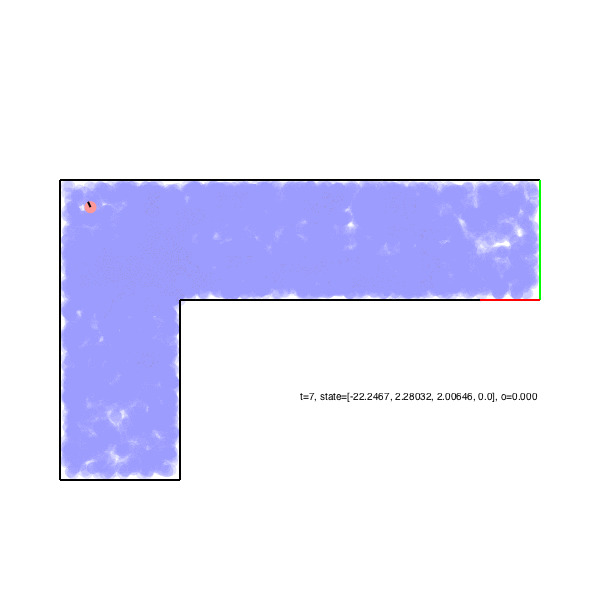
\includegraphics[height=\textheight/8]{roomba_example/pomcpow_analytic_bounds/pomcpow_info_gather_frames/out00097.jpg}}{$t = 97$} &
    \end{tabular}
  \caption{A time lapse of an example trajectory as planned by
           \emph{\ac{pomcpow}-analytic}. The behavior generated by the \ac{pomdp} solver
           performs active information gathering to reduce uncertainty and reaches the
           goal location after $97$ steps.}
  \label{fig:pomcpow-analytic-infogather}
\end{figure}

\begin{figure}[htpb]
    \centering
    \begin{tabular}{ccc}
      \subf{\includegraphics[height=\textheight/8]{roomba_example/mlmpc/mlmpc_stuck_frames/out00000.jpg}}{$t = 0$} &
      \subf{\includegraphics[height=\textheight/8]{roomba_example/mlmpc/mlmpc_stuck_frames/out00010.jpg}}{$t = 10$} &
      \subf{\includegraphics[height=\textheight/8]{roomba_example/mlmpc/mlmpc_stuck_frames/out00020.jpg}}{$t = 20$}\\
      \hline \\
      \subf{\includegraphics[height=\textheight/8]{roomba_example/mlmpc/mlmpc_stuck_frames/out00030.jpg}}{$t = 30$} &
      \subf{\includegraphics[height=\textheight/8]{roomba_example/mlmpc/mlmpc_stuck_frames/out00040.jpg}}{$t = 40$} &
      \subf{\includegraphics[height=\textheight/8]{roomba_example/mlmpc/mlmpc_stuck_frames/out00050.jpg}}{$t = 50$}\\
      \hline \\
      \subf{\includegraphics[height=\textheight/8]{roomba_example/mlmpc/mlmpc_stuck_frames/out00060.jpg}}{$t = 60$} &
      \subf{\includegraphics[height=\textheight/8]{roomba_example/mlmpc/mlmpc_stuck_frames/out00070.jpg}}{$t = 70$} &
      \subf{\includegraphics[height=\textheight/8]{roomba_example/mlmpc/mlmpc_stuck_frames/out00080.jpg}}{$t = 80$}\\
      \hline \\
      \subf{\includegraphics[height=\textheight/8]{roomba_example/mlmpc/mlmpc_stuck_frames/out00090.jpg}}{$t = 90$} &
      \subf{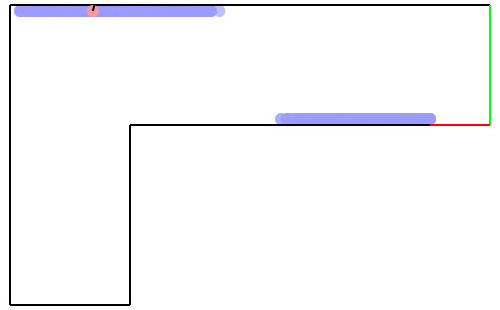
\includegraphics[height=\textheight/8]{roomba_example/mlmpc/mlmpc_stuck_frames/out00100.jpg}}{$t = 100$} &
      \subf{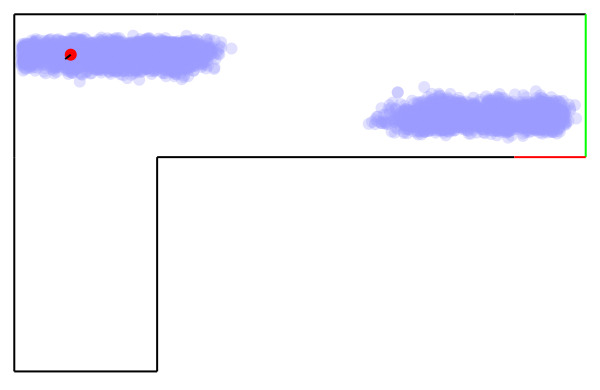
\includegraphics[height=\textheight/8]{roomba_example/mlmpc/mlmpc_stuck_frames/out00110.jpg}}{$t = 110$}\\
      \hline \\
      \subf{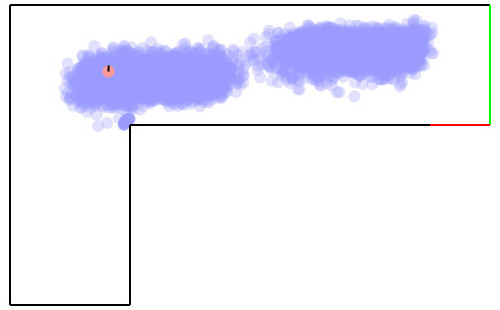
\includegraphics[height=\textheight/8]{roomba_example/mlmpc/mlmpc_stuck_frames/out00120.jpg}}{$t = 120$} &
      \subf{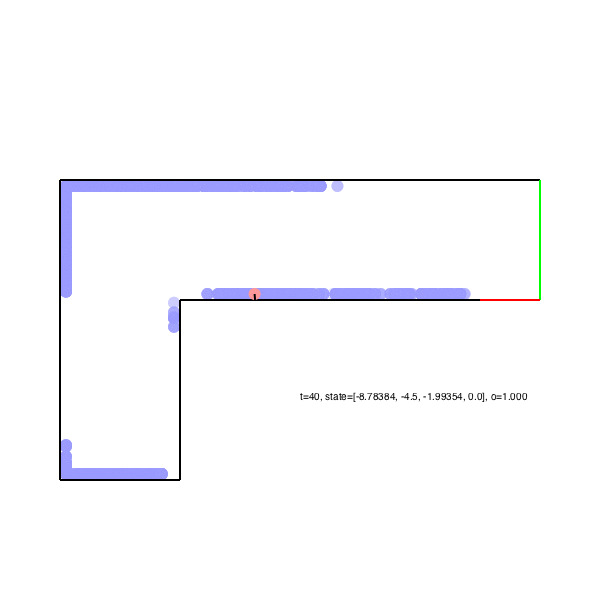
\includegraphics[height=\textheight/8]{roomba_example/mlmpc/mlmpc_stuck_frames/out00130.jpg}}{$t = 130$} &
      \subf{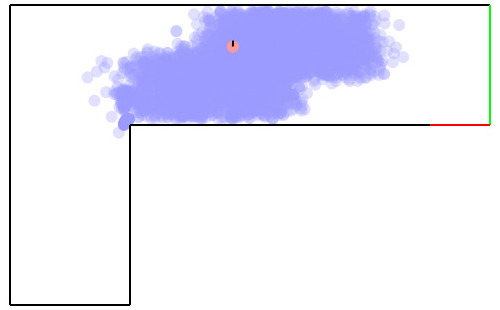
\includegraphics[height=\textheight/8]{roomba_example/mlmpc/mlmpc_stuck_frames/out00140.jpg}}{$t = 140$}\\
    \end{tabular}
\caption{A time lapse of an example trajectory where planning with \ac{mlmpc}
         leads to an oscillating decision  when using the same initial
         conditions and random seed as in the simulation run shown in
         \Cref{fig:mlmpc-oscillating}. The trajectory is truncated after $140$
         steps as it fails to reach a successful terminal state within the
         simulation horizon.}
  \label{fig:mlmpc-oscillating}
\end{figure}




%###########################################################################
\end{appendix}
